\documentclass{scutthesis} % 不填充空白页。如果需要双面打印版,请注释掉本行并启用下一行
%\documentclass[print-both-sides]{scutthesis} % 使用双面打印版(填充额外空白页以保证每一章开头都在奇数页)


\etitlefirst{}
\etitlesecond{}

% 论文中文标题
\ctitle{基于卷积神经网络的手写数字及写字人识别}

% 作者详细信息
\cauthor{王\ 小\ 明}        % 作者姓名
\studentid{12350004}       % 学号
\cschool{计算机学院}        % 学院
\cclass{计算机一班}         %班级
\cmajor{计算机科学与技术}    %专业
\cyear{2024}               %毕业年份


% 指导老师信息
\cmentor{王大明 \ (教授)}


\cabstract{

    关键词4个左右,每个关键词用中文的分号“;”隔开,最后一个关键词不用分号。汉字摘要字数一般不超过300字,英文摘要约1200字符。

    其中'\textbackslash cabstract'为中文摘要,'\textbackslash eabstract'为英文摘要。每个关键词用中文的分号隔开,最后一个关键词不打标点符号。

}
\ckeywords{多变量系统;预测控制;环境试验设备}

\eabstract{
    % 英文摘要及关键词内容应与中文摘要及关键词内容相同。中英文摘要及其关键词各置一页内。
    英文摘要内容要与中文摘要表达意思一致。
    Artificial Neuron Network (ANN) simulates human being's brain function and build the network structure. Convolutional Neural Network (CNN) have many advantage, such as ……
    (2) This paper introduces the common pretreatment method of image, such as collecting image, normalization, graying and binarization. And apply these to the handwritten numeral recognition experiment and handwritten numerals writer recognition experiments.

}
% 英文文关键词(每个关键词之间用,分开, 最后一个关键词不打标点符号。)
\ekeywords{Writer recognition;Convolutional Neural Network;Handwritten character recognition关键字首字母大写}

\pagestyle{empty}

\begin{document}
% 论文前置部分
\frontmatter
\pagenumbering{Roman}
\makeUndergraduateCover    % 生成封面

\makedisclaim % 生成不带签名的原创性声明和版权使用授权书

\maketableofcontents        % 生成目录

\makeabstract       % 生成中英文摘要
% \makelistoffiguretable % 生成图表目录
% 论文主体部分
\mainmatter
% 引言
% 正文
\chapter{引言}
引言部分建议内容:课题的背景与意义;相关研究综述;本课题的主要研究内容;论文组织结构等部分。
\section{课题的背景与意义}
\subsection{理工科论文要求}
理工类毕业论文或设计说明书中一般包括任务的提出,方案论证或文献综述,设计与计算(可分为总体设计和单元设计几部分)说明,试验调试及结果的分析,结束语等内容。理工类毕业论文字数一般要求在一万字以上,对于工程设计和软件开发与仿真等类型的毕业设计,由于绘图或计算机编程工作量较多,论文字数可适当减少。要求理论依据充分,数据准确,公式推导及计算结果正确。

为了使学生在技术经济分析能力方面得到锻炼,凡涉及到应用于实际中产生经济效果的毕业设计(论文),如理工类的工程设计型、产品开发型、软件开发与仿真型和管理等类型的毕业设计(论文),都要进行技术经济分析。

\section{相关研究综述}
注意事项:禁止将网页上的内容直接拷贝到本文档中,一方面会破坏论文模板格式(增加了很多额外的格式),另一方面网页中有很多非打印字符,在显示所有隐藏格式时,这些非打印字符一览无余,会被质疑该论文有抄袭嫌疑。一般的做法是先将网页内容拷贝到记事本文档,再从记事本文档拷贝过来,这样就能消除网页格式,再在此基础上进行修改。

\textbf{综述注意事项:}文献要按顺序引用,文献列表中未被正文引用到的文献应该删除掉。另外文献不少于10篇,其中外文文献至少有一篇(官方2篇)。

\section{本课题的主要研究内容}
本课题的主要研究内容\\
\section{论文组织结构}
论文组织结构\\
\newpage

\chapter{\LaTeX 模板使用说明}
\section{论文信息的输入和封面的自动生成}
在开始使用本模板前,应该开头位置输入相应的论文相关信息,模板会根据信息自动生成目录和诚信承诺书。如图\ref{author}。
\begin{figure}[htbp]
        \centering
        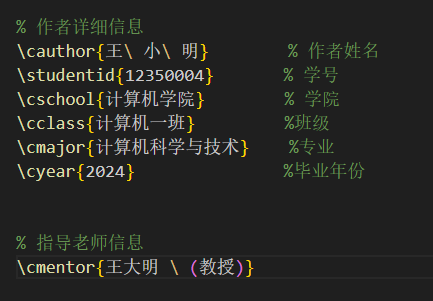
\includegraphics[height=6.54cm]{image/作者信息.png}
        \caption{论文信息}
        \label{author}
\end{figure}

\section{标题的使用}
标题的使用可见图\ref{til}。其中,一级标题通过\textbackslash chapter\{\}。二级标题通过 \textbackslash section\{\}。三级标题通过\textbackslash subsection\{\}。
\begin{figure}[htbp]
        \centering
        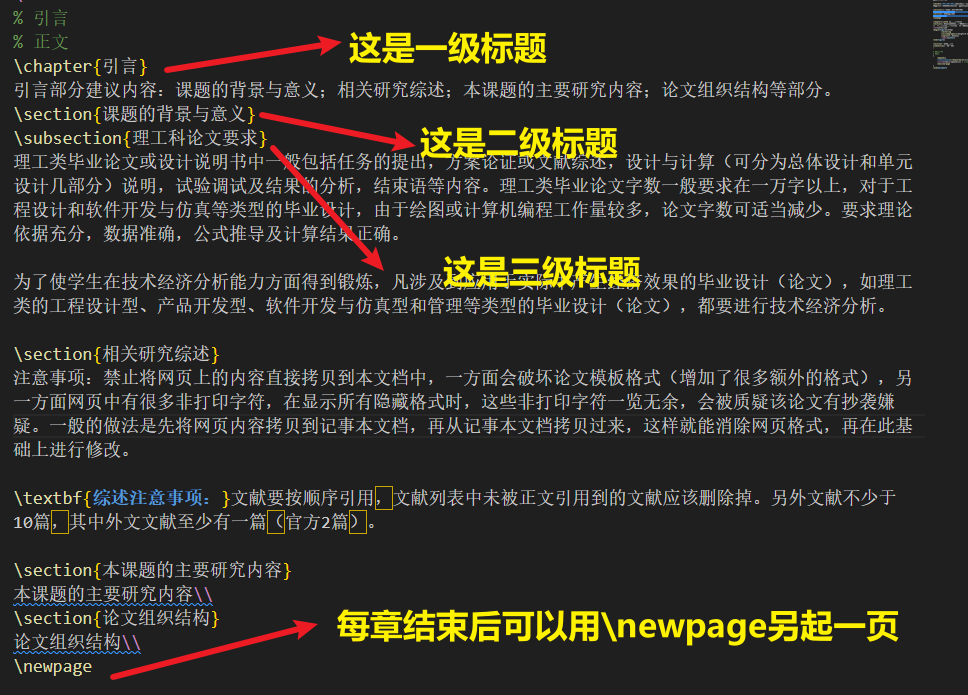
\includegraphics[width=0.65\linewidth]{image/标题使用.png}
        \caption{标题使用}
        \label{til}
\end{figure}

\section{表格的使用}
表格的使用可以通过 \textbackslash table\{\}。详细说明如图\ref{tablea}所示。
\begin{figure}[htbp]
        \centering
        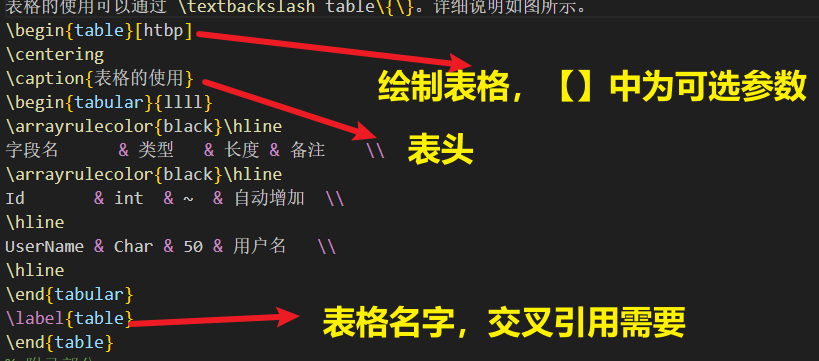
\includegraphics[width=0.65\linewidth]{image/table.png}
        \caption{表格使用}
        \label{tablea}
\end{figure}

通过绘制我们可以得到表如表\ref{table}所示。
\begin{table}[htbp]
\centering
\caption{表格的使用}
\begin{tabular}{llll} 
\arrayrulecolor{black}\hline
字段名      & 类型   & 长度 & 备注    \\ 
\arrayrulecolor{black}\hline
Id       & int  & ~  & 自动增加  \\ 
\hline
UserName & Char & 50 & 用户名   \\
\hline
\end{tabular}
\label{table}
\end{table}

\section{公式的使用}
\begin{equation}
    q+q = 2q
    \label{gongshi}
\end{equation}
公式可通过 \textbackslash begin\{ equation \}使用,引用可通过\textbackslash label,具体操作下文会提及。

\section{图片的插入和交叉引用}
\subsection{图片的使用}
图片的使用可通过\textbackslash begin\{figure\}实现,其中[htbp]可控制图片位置。见图\ref{pic}。
\begin{figure}[htbp]
        \centering
        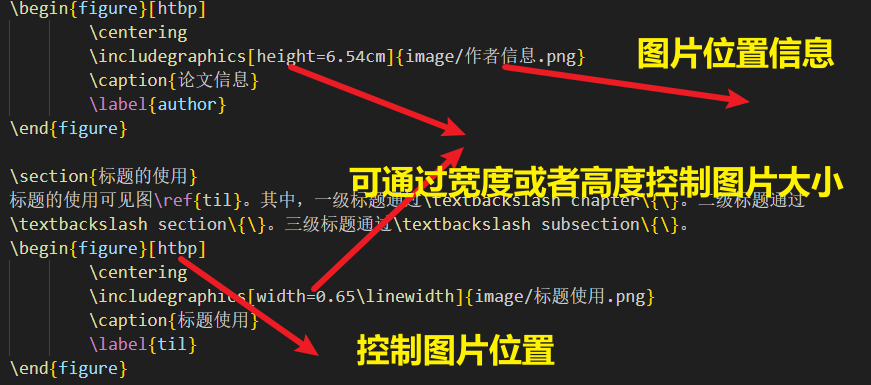
\includegraphics[width=0.65\linewidth]{image/figure.png}
        \caption{图片使用}
        \label{pic}
\end{figure}

\subsection{多图排版样例}
本章节提供几个多图摆放的样例。
\begin{figure}[htbp]
\begin{minipage}[t]{0.48\linewidth}
\centering
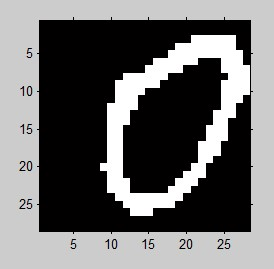
\includegraphics[width=0.9\textwidth]{image/chap04/1.jpg}
\caption{图1-1裂缝对照图}
\label{fig:side:a}
\end{minipage}%
\begin{minipage}[t]{0.48\linewidth}
\centering
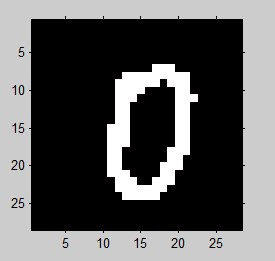
\includegraphics[width=0.9\textwidth]{image/chap04/2.jpg}  % 2.2in
\caption{图1-2裂缝对照图}
\label{fig:side:b}
\end{minipage}
\end{figure}


\begin{figure}[!htp]
	\centering
	\subfloat[附件一中图1-2]{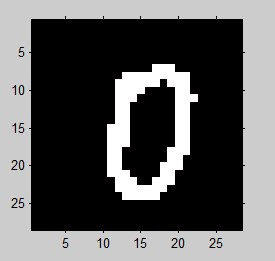
\includegraphics[width=0.4\textwidth]{image/chap04/2.jpg}}\qquad
	\subfloat[附件一中图1-8]{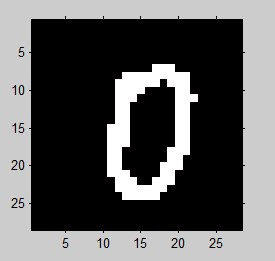
\includegraphics[width=0.4\textwidth]{image/chap04/2.jpg}} \\
	\caption{高斯模糊降噪后图像对比}
    \label{cpm-1}
\end{figure}

\subsection{交叉引用}
在\LaTeX 中,我们可以通过\textbackslash ref\{\}来对任何表格、图片、章节等进行引用。我们\textbackslash label 来对这些需要引用的命名,再在正文中通过 \textbackslash ref\{XX\}来进行引用。例如\ref{fig:side:a},\ref{author}。但是这种方式不能自动识别图表公式,需要自行添加“图”。

已定义自动引用格式,所有引用图片、公式、表格等内容均使用同一个命令`\textbackslash autoref\{\}`进行引用,该命令将会自动产生例如` 式``图 `等前置词语。例如\autoref{cpm-1},\autoref{author}。
\newpage

\chapter{参考文献说明}
参考文献的著录方法采用我国国家标准GB7714-87《文后参考文献著录规则》中规定采用的“顺序编码制”,中外文混编。论文中,引用出处按引用先后顺序用阿拉伯数字和方括号“[]”放在引文结束处最后一个字的右上角作为对参考文献表相应条目的呼应。文后参考文献表中,各条文献按在论文中的文献序号顺序排列。

参考文献引用,需按顺序引用,可利用交叉引用。其引用的文献,需采用上标字体,具体格式已在本文档做好,选中引用部分。\overcite{ref1,ref2}

参考文献均使用 bibtex 的形式记录在`main.bib`文件中,当需要引用时可使用`\textbackslash cite`和`\textbackslash overcite\`两个命令引用,前者为引用符号处于文本基线,后者为上标形式。


\newpage

\backmatter
\renewcommand{\chaptermark}[1]{\markboth{\songti #1}{}}
\chapter{致谢}

四年时间转眼即逝,青涩而美好的本科生活快告一段落了。回首这段时间,我不仅学习到了很多知识和技能,而且提高了分析和解决问题的能力与养成了一定的科学素养。虽然走过了一些弯路,但更加坚定我后来选择学术研究的道路,实在是获益良多。这一切与老师的教诲和同学们的帮助是分不开的,在此对他们表达诚挚的谢意。

最后我要感谢我的家人,正是他们的无私的奉献和支持,我才有了不断拼搏的信心和勇气,才能取得现在的成果。

\vskip 108pt
\begin{flushright}
    王小明\makebox[1cm]{} \\
    \today
\end{flushright}

\newpage
\makereferences
\newpage
\appendix
\renewcommand{\chaptermark}[1]{\markboth{\songti  附录\thechapter\ ~#1}{}}

\chapter{补充更多细节}

\section{补充图}

\subsection{补充图}

\newclearpage
\chapter{附录2}

\end{document}